% -*- TeX -*- -*- UK -*- -*- BMR -*-
% ----------------------------------------------------------------
% Beamer presentation ************************************************
% **** -----------------------------------------------------------
\documentclass{beamer}%[hyperref={backref=slide}]

\usepackage{array}
\input{sl_slide_preamble.tex}
%\input{sl_slide_preamble_nonotes.tex}
\input{sl_slide_graphics_preamble.tex}
\input{sl_definitions.tex}
\input{sl_slide_symbols.tex}
%
\graphicspath{{"Figs/"}}
\DeclareMathOperator{\SNR}{SNR}
\DeclareMathOperator{\snr}{SNR}
%matrices
\newcommand{\inv}{^{-1}}
\newcommand{\I}{\mathbf{I}}
%prob vector
\newcommand{\pr}{\mathbf{p}}
%equilibrium distribution
\newcommand{\eq}{\pr^\infty}
%first passage times
\newcommand{\fpt}{\mathbf{T}}
%off-diag first passage times
\newcommand{\fptb}{\overline{\fpt}}
%other symbols
\newcommand{\w}{\mathbf{w}}
\newcommand{\W}{\mathbf{W}}
\newcommand{\frg}{\W^\mathrm{F}}
\newcommand{\M}{\mathbf{M}}
\newcommand{\F}{\boldsymbol{\Phi}}
\newcommand{\wv}{\vec{w}}
%super/subscripts
\newcommand{\pot}{^{\text{pot}}}
\newcommand{\dep}{^{\text{dep}}}
\newcommand{\potdep}{^{\text{pot/dep}}}
\newcommand{\lmax}{_{\text{max}}}
\newcommand{\lmin}{_{\text{min}}}
%quantities
\newcommand{\initial}{\mathcal{I}}
\newcommand{\area}{\mathcal{A}}
\newcommand{\CS}{\mathcal{S}}
\newcommand{\comp}{^\mathrm{c}}
\renewcommand{\e}{\mathsf{e}}
%---------Title-----------------------------------------------------------

\title[Saturation by enh. plasticity impairs learning]{A saturation model for impaired learning with enhanced plasticity}
%
\subtitle{\small{based on work in preparation by: T.D. Barbara Nguyen-Vu, Grace Q. Zhao, Han-Mi Lee, SL, Surya Ganguli, Carla J. Shatz, Jennifer L. Raymond
}}
%
\author{Subhaneil Lahiri%\inst{1}
}
%
\institute[Stanford]{%
%\inst{1}
Stanford University, Applied Physics
}
%
%\slideCaption{}

%---------Beginning--------------------------------------------------------

\begin{document}

%-------------Slide--------------------------------------------------------

\begin{frame}
%
 \titlepage
%
\end{frame}

%-------------Slide--------------------------------------------------------

\begin{frame}{Outline}
%
 \tableofcontents[hideallsubsections]
 %
%
\end{frame}


%-------------Section--------------------------------------------------------

\section{VOR learning and the cerebellum}

%-------------Slide--------------------------------------------------------

\begin{frame}{Vestibular Occular Reflex}
%
 \parbox[t]{0.4\linewidth}{\aligntop{\includegraphics[width=0.99\linewidth]{VOR.svg}}}
 \parbox[t]{0.59\linewidth}{%
 Eye movements compensate for head movements to maintain fixation.
 
 \vp Requires control of $\text{VOR gain} = \frac{\text{eye velocity}}{\text{head velocity}}$.
 
 \vp Needs to be adjusted as eye muscles age, \etc
 }
%
\end{frame}


%-------------Slide--------------------------------------------------------

\begin{frame}{VOR training}
%
 \parbox[t]{0.2\linewidth}{\aligntop{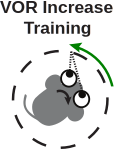
\includegraphics[width=0.99\linewidth]{VORinc.svg}}\\[1cm]
   \note[item]{trick brain into thinking VOR gain needs adjusting my moving visual stimulus}
   \note[item]{anti-phase \lto increase gain}
 \aligntop{
\includegraphics[width=0.99\linewidth]{VORdec.svg}}}
 \note[item]{in phase \lto decrease gain}
 \hspace{0.15\linewidth}
 \parbox[t]{0.59\linewidth}{\aligntop{\includegraphics[width=0.99\linewidth]{VORcircuit.svg}}}
 \note[item]{Gain change involves cerebellum}
 \note[item]{Marr-Albus-Ito: Pf-Pk synapses}
 \note[item]{Lisberger-Miles: Vestibular input-VN synapses}
 \note[item]{Different mechs for different freq, head angle, gain up/down.}
 \note[item]{Different Pk cells have different tunings.}
 \note[item]{Gain up in case of interest: LTD in Pf-Pk in flucculus}
 \note[item]{Gain down: uses different mech for behaviour, but does reverse LTD in Pf-Pk in flucculus}
%
\end{frame}

%-------------Section--------------------------------------------------------

\section{The effects of enhanced plasticity and saturation}


%-------------Slide--------------------------------------------------------

\begin{frame}{Questions}
%
 \begin{itemize}
   \item Can the saturation effect overcome the enhanced plasticity?
   \note[item]{in competition}
   \item How can a little reverse bias help, but too much hurt?
   \note[item]{first makes sense, but second?}
   \item Can we find a purely synaptic explanation of these results?
   \note[item]{This is a question about synaptic populations after all.}
 \end{itemize}
%
\end{frame}

%-------------Section--------------------------------------------------------

\section{Modelling approach}

%-------------Slide--------------------------------------------------------

\begin{frame}{Model of circuit}
%
 %
 \begin{center}
   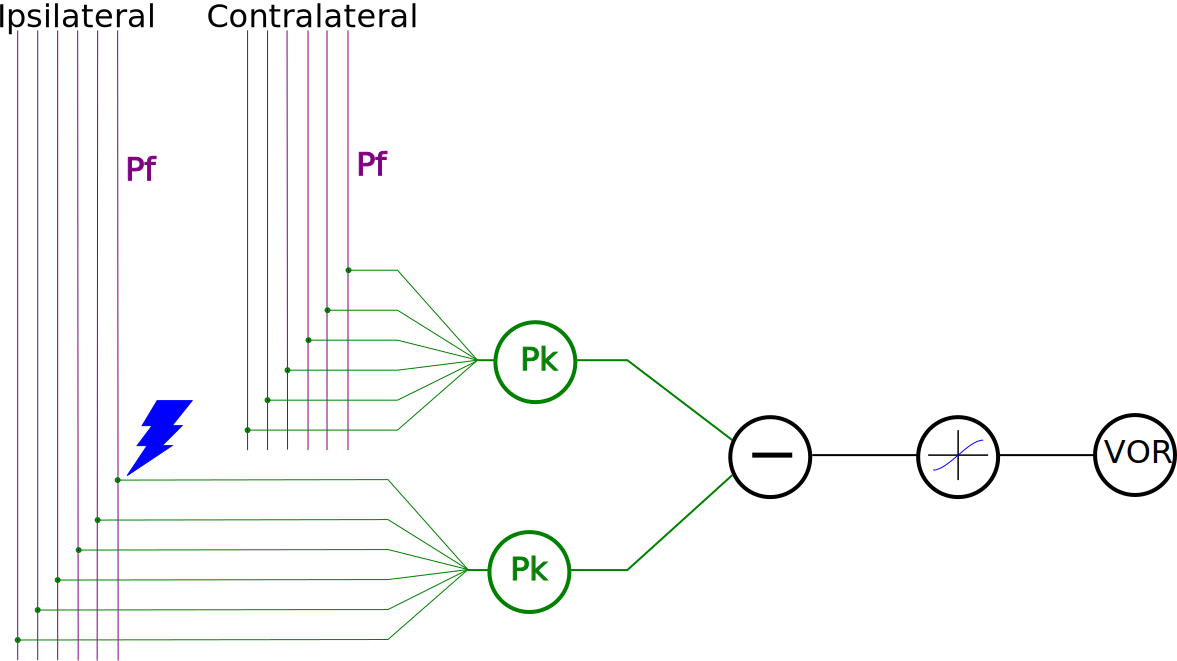
\includegraphics[width=0.9\linewidth]{VORmodel.svg}
 \end{center}
 %
 \note[item]{Contralateral baseline shift compensates for Our baseline shift}
 \note[item]{Gain increase due to LTD at lightning}
 \note[item]{Gain decease due to plasticity elsewhere, but also reverses LTD at lightning.}
 \note[item]{Nonlinearity here won't affect our questions, as long as it doesn't change}
 \note[item]{Nonlinearity before compensation could change things}
%
\end{frame}

%-------------Slide--------------------------------------------------------

\begin{frame}{Simplifying assumptions}
%
\begin{itemize}
  \item No spatial/temporal correlations in plasticity events.
      %
      \note[item]{allows us to concentrate on synapse, not neuron/network}
      %
%  \item Which synapses eligible for plasticity chosen randomly.
      %
      \note[item]{No filing system}
      %
  \item Potentiating/depressing plasticity events $\sim$ Poisson processes.% with rates $rf\potdep$, where $f\pot+f\dep=1$.
      %
      \note[item]{don't care if STDP...}
%      %
%      \note[item]{$r=$ total rate of plasticity events per synapse, $f\potdep=$ fraction of events that are potentiating/depressing.}
      %
  \item Potentiation and depression are described by Markov processes.% with transition probabilities $\M\potdep$.
%      %
%      \note[item]{matrix elements: transition prob from $i\to j$, given pot/dep}
%  \item Ideal observer: read weights directly.
%      \note[item]{not electrical activity: don't model neurons/network}
%      \note[item]{upper bound on electrical activity readout}
%      %
%  \item Synaptic weights can only take values $\pm1$.
      %
  \citerr{Fusi2005cascade,Fusi2007multistate,Barrett2008discrete}
      %
      \note[item]{looks like binary synapse from outside. Inside...}
\end{itemize}
%
\end{frame}

%-------------Slide--------------------------------------------------------

\begin{frame}{Dynamics}
%
  There are $N$ identical synapses with $M$ internal functional states.
  %
  \begin{center}
    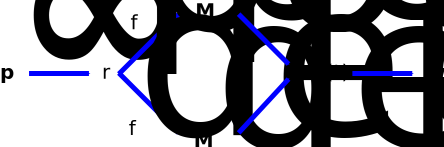
\includegraphics[width=0.7\linewidth]{model.svg}
  \end{center}
  %
  \note[item]{stoch process has steady state.}
  \note[item]{Prior activity puts it in this state. row vec.}
  \note[item]{plasticity events at rate r}
  \note[item]{fraction pot/dep}
  \note[item]{probs changed by Markov matrices, prob $i\to j$}
  \note[item]{Readout: synaptic weight vec when in each state.}
  \vp
% At $t=0$, the memory is created by $\M\potdep$ with probability $f\potdep$.
% \note[item]{for this one, we keep track of pot/dep, look for inc/dec of $\w$}
%
% \vp Forgetting caused by subsequent memories, evolving as
%
  \begin{equation*}
  \begin{aligned}
    \diff{\pr(t)}{t} &= r\pr(t)\frg,
    &\qquad
    \frg &= f\pot\M\pot+f\dep\M\dep-\I,\\&&
    \eq\frg &=0.
  \end{aligned}
  \end{equation*}
%
  \note[item]{Memory at $t=0$, keep track of pot/dep}
  \note[item]{subsequent: average over pot/dep}
% \note[item]{$\frg$ is forgetting matrix, $\I=$identity, don't keep track of pot/dep}
% Eventually, this will settle into the equilibrium distribution:
% %
% %
% \note[item]{In equilibrium prior to memory creation}
%
\end{frame}


%-------------Slide--------------------------------------------------------

\begin{frame}{Modelling VOR learning}
%
\begin{tabular}{>{\bfseries}ll>{\impl}l}
    Mutation: &
    Changes mechanism of LTD  &
    change $\M\dep$.
    \note[item]{lower threshold \lto increase off-diagonal elements.}
 \\[1cm]
    Training: &
    Changes statistics of LTP/LTD  &
    change $r,f\pot,f\dep$.
    \note[item]{Only parameters we have. Don't care about $r$.}
 \\[1cm]
    Learning: &
    Change in VOR gain &
    decrease in $\av{\w}$.
    \note[item]{Only output we have. Don't keep track of synaptic identity.}
\end{tabular}
%
\end{frame}

%-------------Section--------------------------------------------------------

\section{Modelling results}


%-------------Slide--------------------------------------------------------

\begin{frame}{Binary synapse}
%
 %
 \begin{center}
   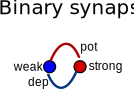
\includegraphics[width=0.15\linewidth]{binary.svg} \\[1cm]
   \aligntop{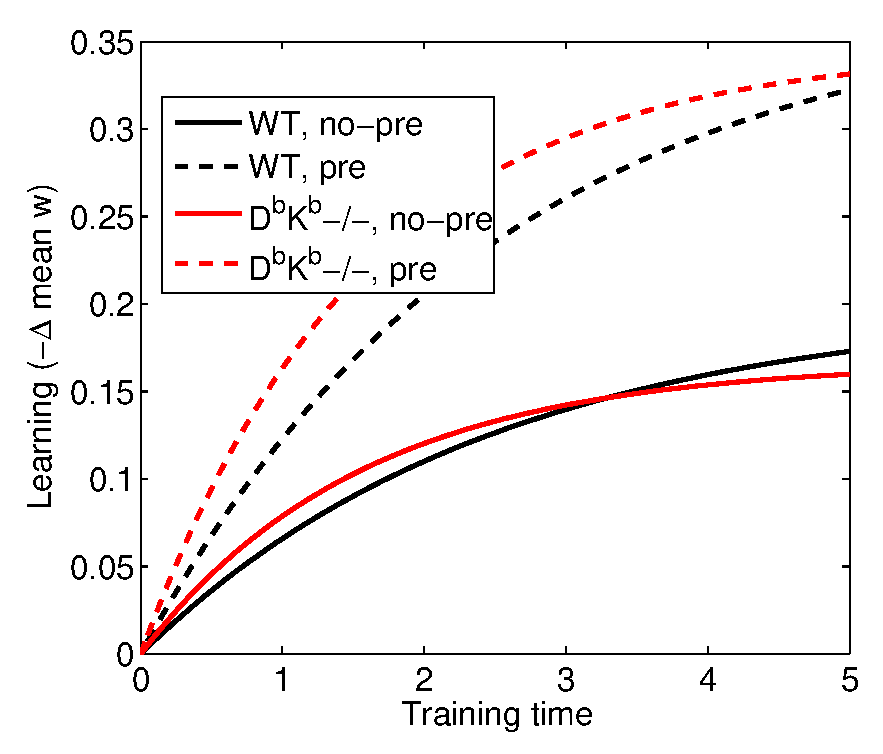
\includegraphics[width=0.35\linewidth]{binary_learnS.eps}}
   \hspace{2cm}
   \aligntop{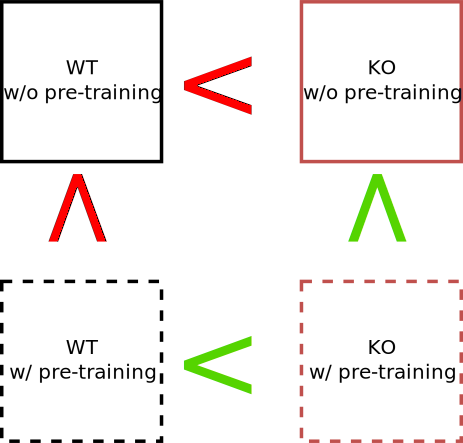
\includegraphics[width=0.35\linewidth]{comparisons_binary.svg}}
 \end{center}
 %
 \note[item]{Compare solid curves}
 \note[item]{Compare black curves}
 \note[item]{understand why next slide}
%
\end{frame}

%-------------Slide--------------------------------------------------------

\begin{frame}{Binary synapse: initial distributions}
%
 %
\adjustbox{valign=m}{\parbox[t]{0.4\linewidth}{
  \begin{raggedleft}
  Learning rate: \phantom{rate of events} \\
  \hp\hp\parbox{0.75\linewidth}{%
  $\sim$ rate of events\\
  $\times$ prob.\ of transition\\
  $\times$ prob.\ ready for $\Delta w$\\
  $\times$ (-$\Delta w$)}
  \end{raggedleft}
}}
% \begin{center}
\alignmid{\parbox[t]{0.5\linewidth}{
 \begin{tabular}{ccc}
   \alignmid{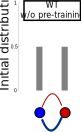
\includegraphics[height=0.5\linewidth]{binary_bar_wt_wo.svg}}
   & \alignmid{\includegraphics[height=0.12\linewidth]{left_bad.svg}} &
   \alignmid{\includegraphics[height=0.5\linewidth]{binary_bar_ko_wo.svg}}
   \\[1.5cm] \alignmid{\includegraphics[height=0.12\linewidth]{up_bad.svg}}
   && \alignmid{\includegraphics[height=0.12\linewidth]{up_good.svg}}\\[0.5cm]
   \alignmid{\includegraphics[height=0.5\linewidth]{binary_bar_wt_w.svg}}
   & \alignmid{\includegraphics[height=0.12\linewidth]{left_good.svg}} &
   \alignmid{\includegraphics[height=0.5\linewidth]{binary_bar_ko_w.svg}}
 \end{tabular}
}}
% \end{center}
 %
 \note[item]{WT: start with everything equal -- just for illustration, not essential}
 \note[item]{WT: during training, increase $f\dep$ (green arrow) $\to$ weakening.}
 \note[item]{KO: inc $q\pot\to$ bias}
 \note[item]{KO: competition between inc prob trans \& dec prob ready}
 \note[item]{KO: first one wins. see why after next model}
 \note[item]{pre: reduces/reverses bias. always helps.}
%
\end{frame}

%-------------Slide--------------------------------------------------------

\begin{frame}{Serial synapse}
%
 %
 \begin{center}
   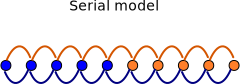
\includegraphics[width=0.5\linewidth]{serial.svg} \\[1cm]
 \note[item]{Still looks binary from outside. Hidden states (not essential).}
 \note[item]{Only see $\Delta w$ at boundary.}
   \aligntop{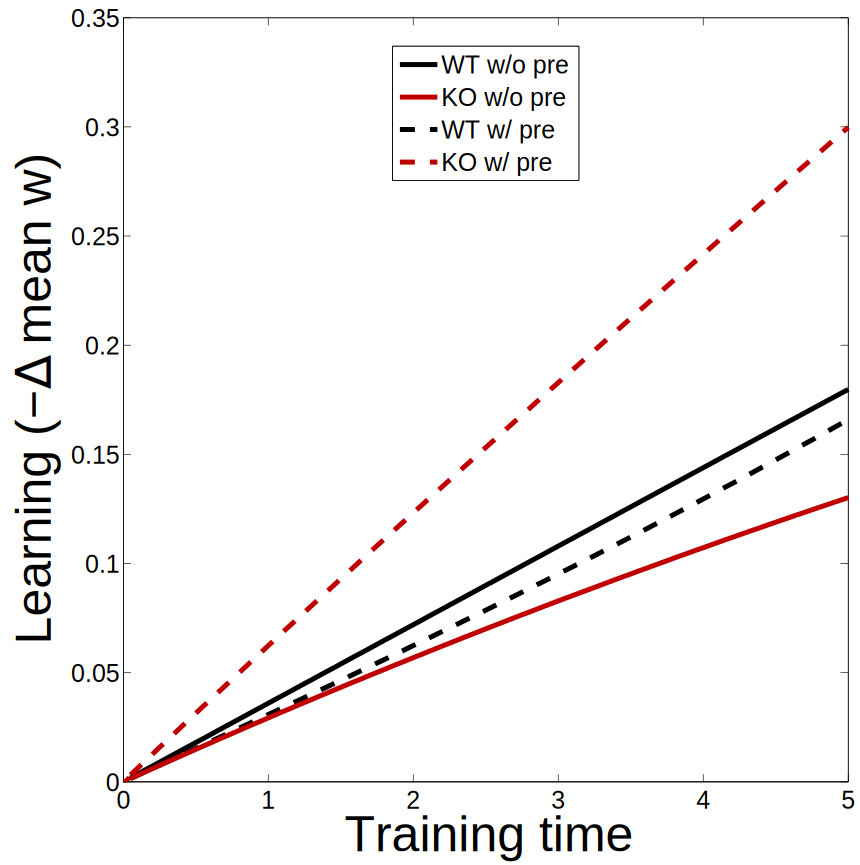
\includegraphics[width=0.35\linewidth]{serial_learnS.eps}}
   \hspace{2cm}
   \aligntop{\includegraphics[width=0.35\linewidth]{comparisons_serial.svg}}
 \end{center}
 %
 
 \note[item]{understand why next slide}
%
\end{frame}

%-------------Slide--------------------------------------------------------

\begin{frame}{Serial synapse: initial distributions}
%
 %
 \begin{center}
 \begin{tabular}{ccc}
   \alignmid{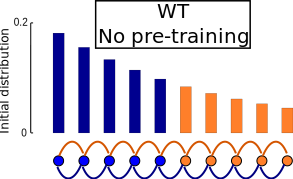
\includegraphics[height=0.19\linewidth]{serial_bar_wt_wo.svg}}
   & \alignmid{\includegraphics[height=0.05\linewidth]{right_good.svg}} &
   \alignmid{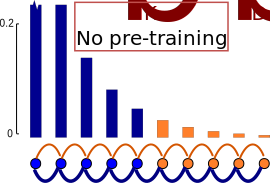
\includegraphics[height=0.19\linewidth]{serial_bar_ko_wo.svg}}
   \\[1.5cm] \alignmid{\includegraphics[height=0.05\linewidth]{down_good.svg}}
   && \alignmid{\includegraphics[height=0.05\linewidth]{up_good.svg}}\\[0.5cm]
   \alignmid{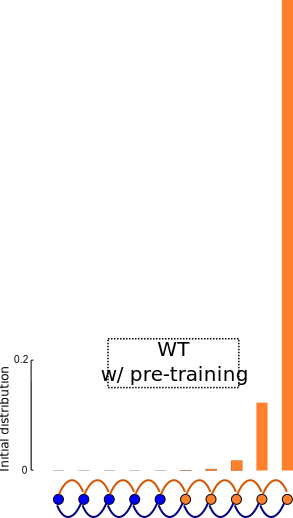
\includegraphics[height=0.19\linewidth]{serial_bar_wt_w.svg}}
   & \alignmid{\includegraphics[height=0.05\linewidth]{left_good.svg}} &
   \alignmid{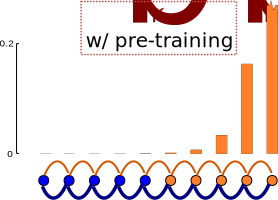
\includegraphics[height=0.19\linewidth]{serial_bar_ko_w.svg}}
 \end{tabular}
 \end{center}
 %
 \note[item]{WT: start with everything equal -- just for illustration, not essential}
 \note[item]{WT: during training, increase $f\dep$ (green arrow) $\to$ weakening.}
 \note[item]{KO: inc $q\pot\to$ bias, now exponential}
 \note[item]{KO: comp. between inc prob trans \& dec prob ready, now only at bndry}
 \note[item]{KO: second one wins, now exponential}
 \note[item]{pre: reduces/reverses bias.}
 \note[item]{pre: little reverse bias repopulates bndry, helps.}
 \note[item]{pre: too much reverse bias moves away from bndry, hurts.}
 \note[item]{maths next slide}
%
\end{frame}


%-------------Slide--------------------------------------------------------

\begin{frame}{Mathematical explanation}
%
 Serial synapse: $\eq_i \sim \CN \prn{\frac{q\pot}{q\dep}}^i$.
 
 \vp Learning rate $\sim \eq_{M/2}\prn{\frac{q\dep}{q\pot}} = \CN \prn{\frac{q\pot}{q\dep}}^{\frac{M}{2}-1}$.
 \note[item]{Detailed balance. Exponential decay.}
 
 \vp For $M>2$: larger $q\dep \implies$ slower learning.
 \note[item]{for large enough $M,q\pot$, overcome $\CN$}
 
 \vp For $M=2$: larger $q\dep \implies$ larger $\CN \implies$ faster learning.
 \note[item]{Other factor in $\eq$ smaller $\implies \CN$ larger.}
%
\end{frame}

%-------------Slide--------------------------------------------------------

\begin{frame}{Essential features}
%
 The success of the serial model relies on two features:
 \begin{itemize}
   \item Enhancing the effect of saturation,
   \note[item]{due to exponential decay}
   \item Metaplasticity -- repeated potentiation makes subsequent depression harder.
   \note[item]{push away from boundary where signal generated}
 \end{itemize}
 %
 \begin{center}
   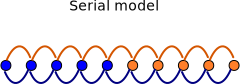
\includegraphics[width=0.4\linewidth]{serial.svg}
 \end{center}
 %
 \note[item]{borne out by other models that fail/succeed}
%
\end{frame}

%-------------Slide--------------------------------------------------------

\begin{frame}{Other models that fail}
%
 \begin{tabular}{ll}
   % & for next tab, \\ for new line...
    \aligntop{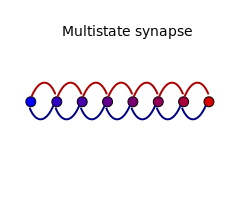
\includegraphics[width=0.4\linewidth]{multistate.svg}}\hspace{1.5cm} &
    \aligntop{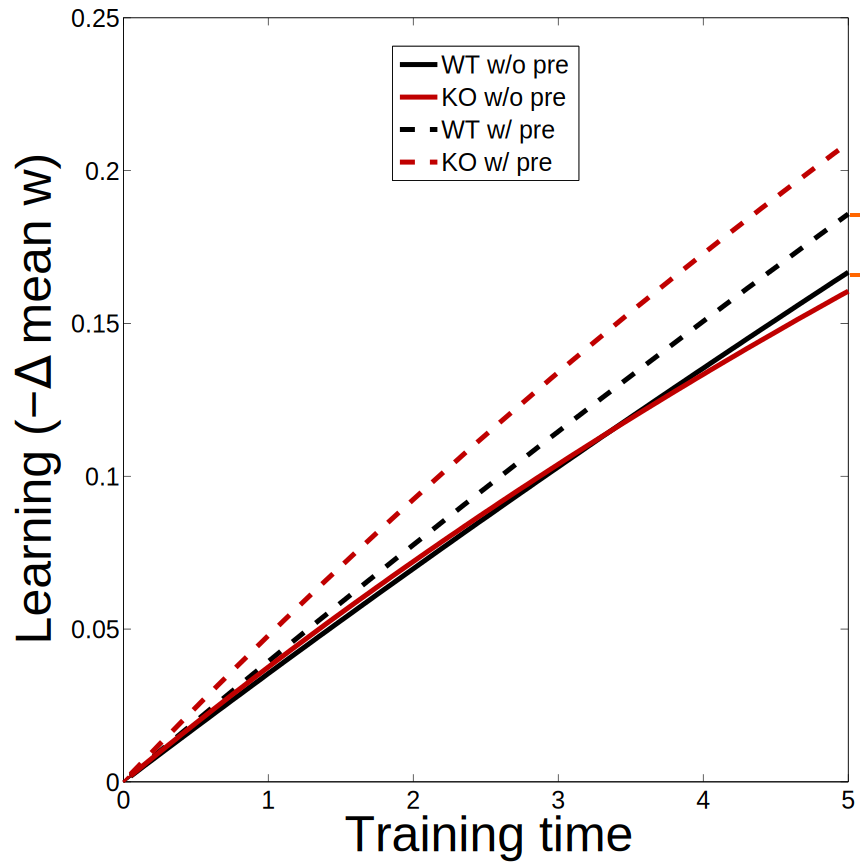
\includegraphics[width=0.28\linewidth]{multistate_learnS.eps}}
    \note[item]{MS: linear weights, unlike serial.}
    \note[item]{like bunch of binary synapses in series.}
    \note[item]{solid curves: fails early on , but catches up quickly}
    \note[item]{black curves: fails badly}
    \note[item]{No real enhancement of saturation, no metaplasticity.}
    \note[item]{All transitions contribute: pushing to end has little effect.}
    \\[2cm]
    \aligntop{\includegraphics[width=0.4\linewidth]{pooled.svg}} &
    \aligntop{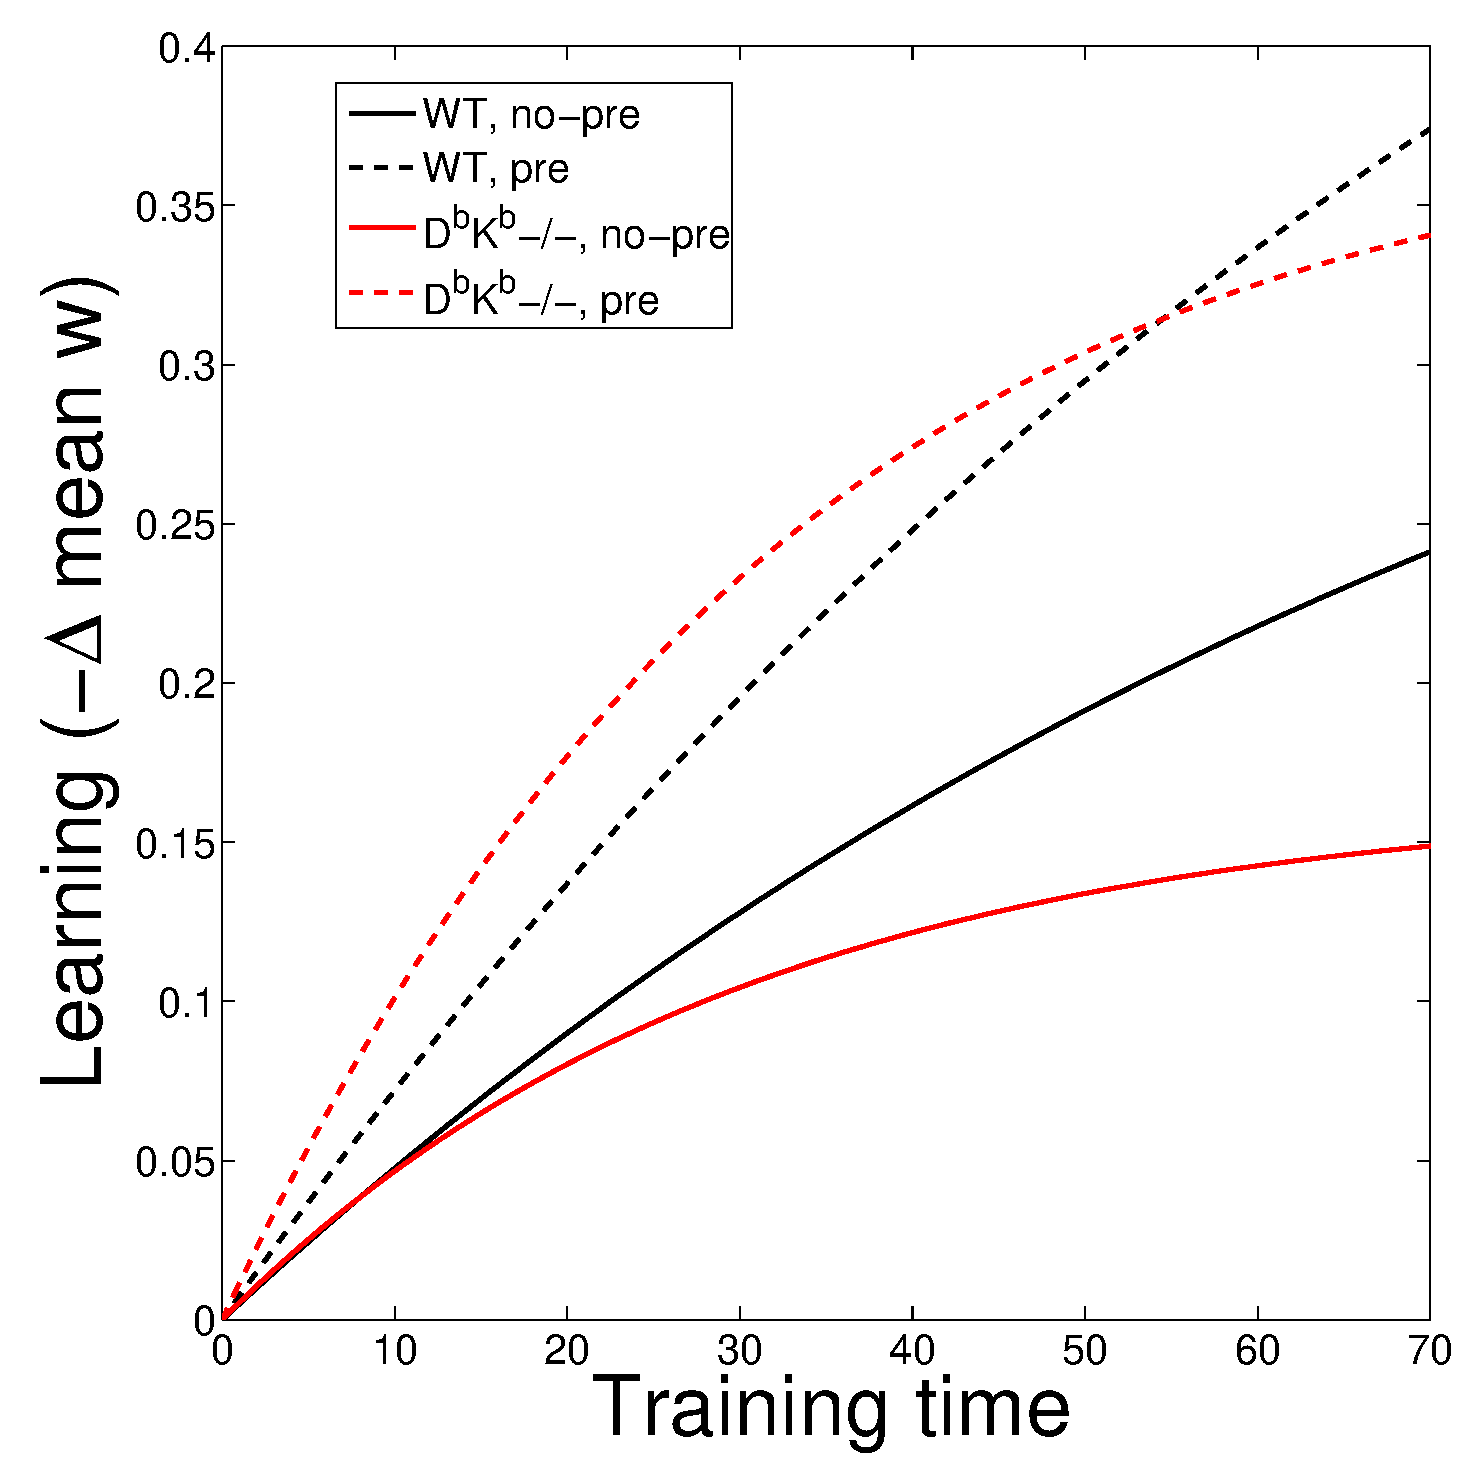
\includegraphics[width=0.28\linewidth]{pooled_scarce_learnS.eps}}
    \note[item]{Pooled: resource depleted by pot/dep. replenished by reverse.}
    \note[item]{solid curves succeed: enhanced saturation}
    \note[item]{black curves fail: opposite metaplasticity, pot makes dep easier}
 \end{tabular}
 
 \citerr{amit1994learning}
%
\end{frame}

%-------------Slide--------------------------------------------------------

\begin{frame}{Other models that work}
%
 \begin{tabular}{ll}
   % & for next tab, \\ for new line...
    \aligntop{\includegraphics[width=0.4\linewidth]{multistate_nonuni.svg}}\hspace{1.5cm} &
    \aligntop{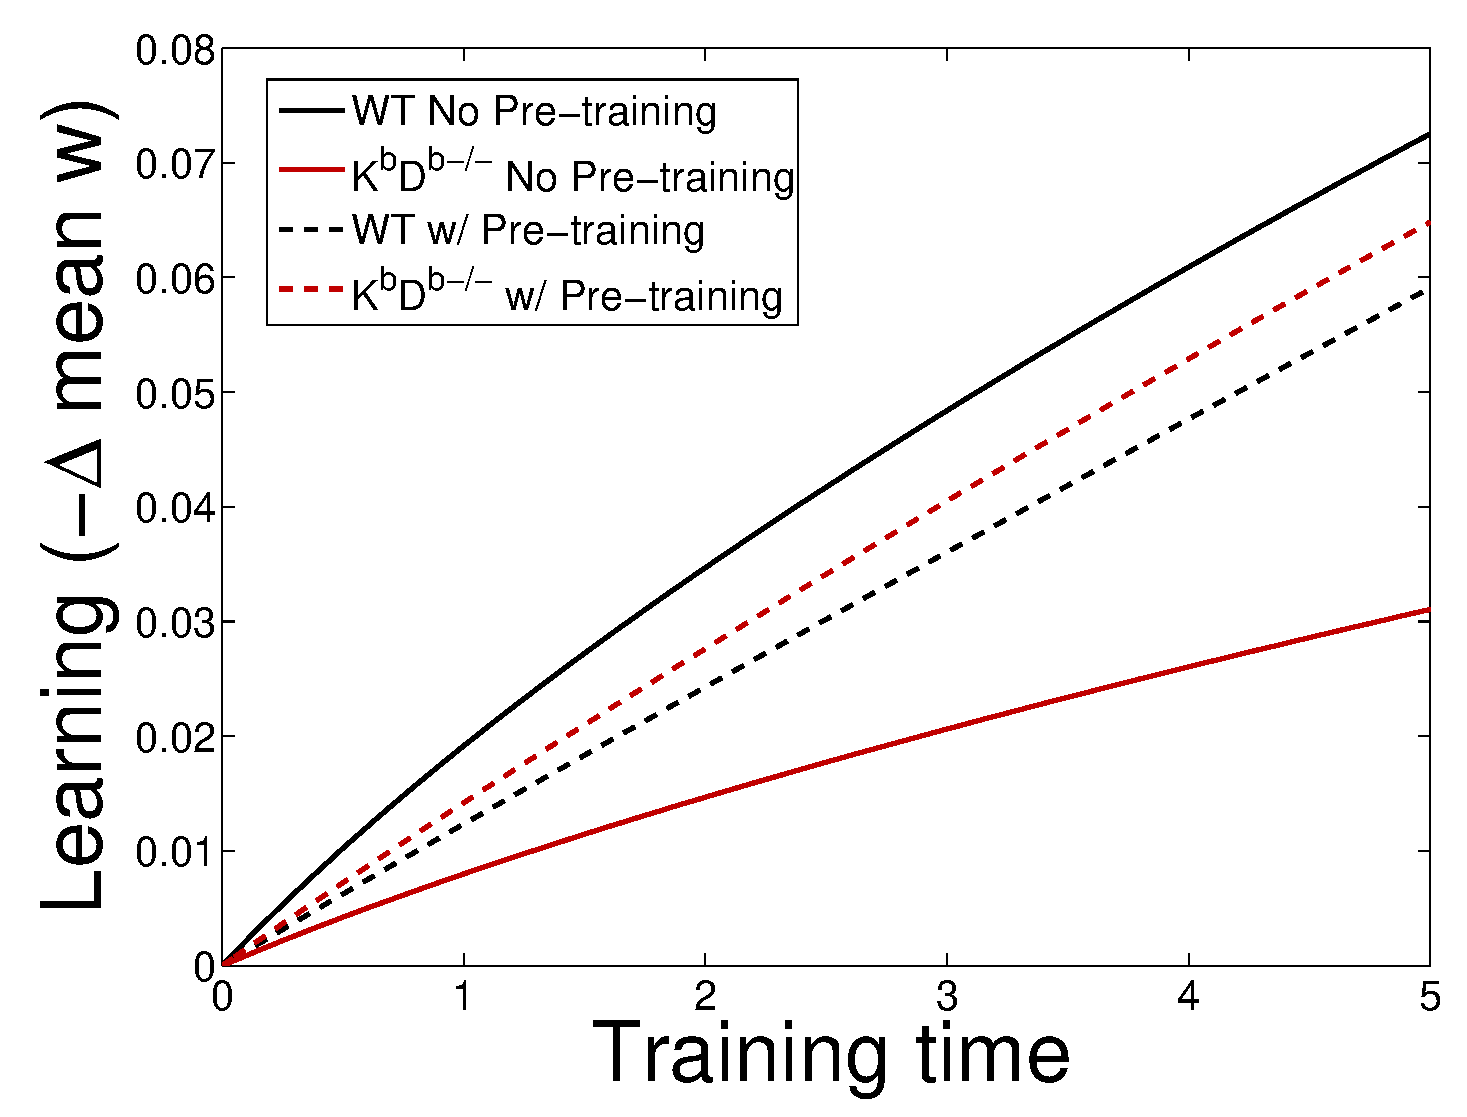
\includegraphics[width=0.28\linewidth]{nonuni_learnS.eps}} \\[2cm]
    \aligntop{\includegraphics[width=0.4\linewidth]{cascade.svg}} &
    \aligntop{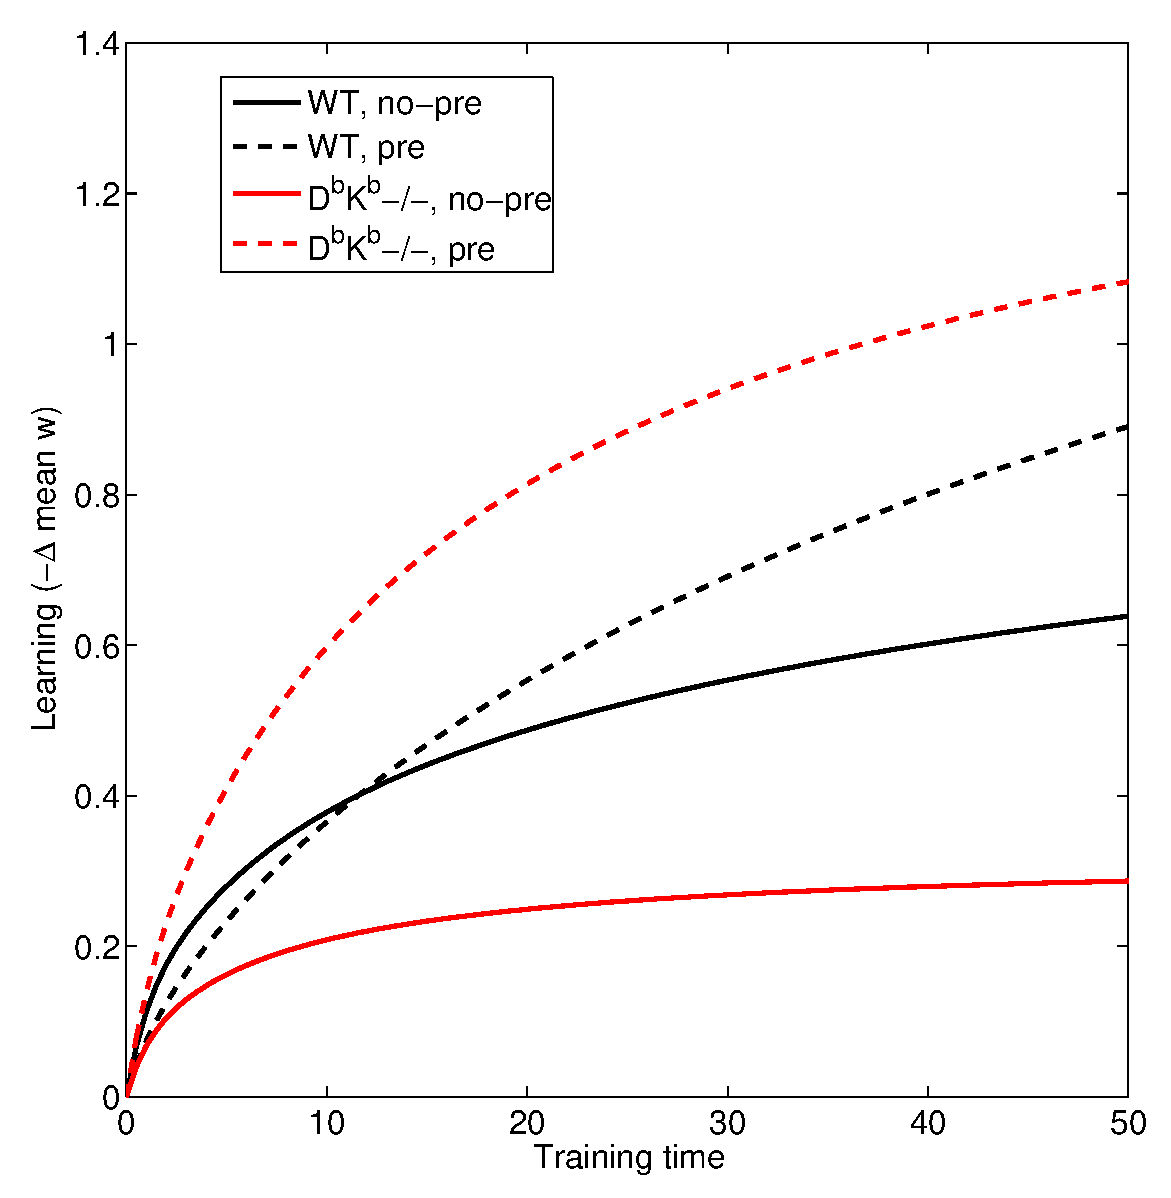
\includegraphics[width=0.28\linewidth]{cascade_long_learnS.eps}}
 \end{tabular}
 \note[item]{Both models, trans probs decay exponentially from centre.}
 \note[item]{Nonuni: linear weights. Cascade: binary weights.}
 \note[item]{Enhanced saturation and metaplasticity}
 \note[item]{Pushing to end makes pot and dep harder}
 \note[item]{Note: hidden states not necessary}
 
 \citerr{Fusi2005cascade}
%
\end{frame}

%-------------Slide--------------------------------------------------------

\begin{frame}{Conclusions and further questions}
%
 \begin{itemize}
   \item The saturation effect overcome the enhanced plasticity, if it is enhanced.
   \alert{Requires complexity}
   \note[item]{\eg exponential deacy, resource depletion,\ldots}
   \item A little reverse bias can help, but too much hurts, if repeated potentiation makes depression harder.
   \alert{Requires metaplasticity}
   \note[item]{\eg moving away from weight boundary, or weaker transitions.}
   \item We can find a purely synaptic explanation of VOR behaviour, iff the synapses have these features. 
   \note[item]{Other explanations? Non-linearity in PK cell?}
   \item We used behaviour to constrain molecular structure of synapses!
   \item Can we constrain it further with more experiments?
 \end{itemize}
%
\end{frame}

%-------------Slide--------------------------------------------------------

\begin{frame}[allowframebreaks]{References}
%

 {\small
 \bibliographystyle{unsrt_slides}
 \bibliography{maths,neuro}
 }
%
\end{frame}


%-----End----------------------------------------------------------------

\end{document}

